% 2011 年浙江卷文科第 22 题：抛物线 x^2=y、圆 x^2+(y+3)^2=1、直线 y=-3。
% 来源 PDF：普通高考/2011/2011浙江文.pdf，SHA-256 36931500dfd850579d93f0a685f0ccea25065c84c09db5157c451093d53b56f0。
% 原页：第 2 页第 3 栏，书页码 712。示意图。
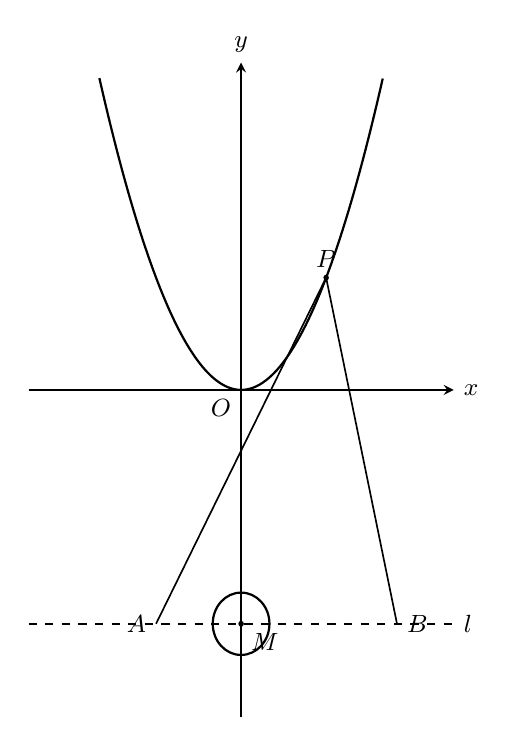
\begin{tikzpicture}[>=stealth, semithick, font=\small, scale=0.9, yscale=1.1]
  \draw[->] (-3,0)--(3,0) node[right] {$x$};
  \draw[->] (0,-4.2)--(0,4.2) node[above] {$y$};
  \draw[thick, domain=-2:2, samples=100] plot (\x,{\x*\x});
  \draw[thick] (0,-3) circle (0.4);
  \fill (0,-3) circle (1.1pt) node[below right] {$M$};
  \draw[dashed] (-3,-3)--(3,-3) node[right] {$l$};
  \coordinate (P) at (1.2,1.44);
  \fill (P) circle (1.1pt) node[above] {$P$};
  \draw (P)--(-1.2,-3) node[left] {$A$};
  \draw (P)--(2.2,-3) node[right] {$B$};
  \node[below left] at (0,0) {$O$};
\end{tikzpicture}
